\scanpage{18}
\mspage{17}

Ceci \unsure{vu|or}, on voit que $(A,\beta)$ définit une structure de maille à \inserted{\uline{un}} \uline{noeud} $A$, à \unsure{birive} $\beta$ \deleted{$\unsure{\epsilon}$}, \unsure{ssi} $(\overline X,\{A_\rho,A_{\rho'}\})$ est une \uline{ficelle} top.

Orienter la maille, c'est par définition orienter la ficelle, i.e. choisir $A_\rho$ ou $A_{\rho'}$, i.e. choisir $\rho$ ou $\rho'$ i.e. une des rives qui constituent la birive.
\margin{\uline{NB} \unsure{Dans tout ce qui précède} \unsure{se réduire au cas} $A_1,A_2$ réduits à un point\ldots}

\deleted{On dit que deux structures de}
Considérons deux \deleted{\unsure{struc}} structures de mailles $(A_1,\underbrace{(\rho_1,\rho'_1)}_{\beta_1})$ et $(A_2,\underbrace{\{\rho_2,\rho'_2\}}_{\beta_2})$ sur $X$.

\figure{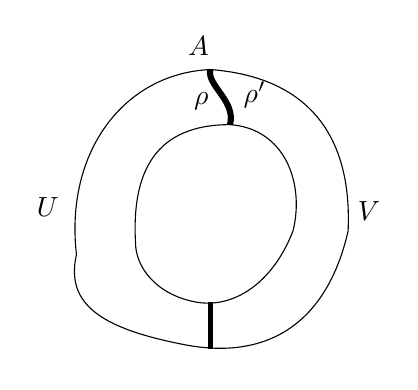
\begin{tikzpicture}[x=1cm,y=1cm]
\draw (0,0) .. controls (-.15,1.3) and (.6,2.3) .. (1.7,2.35) .. controls (3,2.25) and (3.5,1.45) .. (3.45,.3) .. controls (3.2,-.8) and (2.5,-1.35) .. (1.4,-1.15) .. controls (.35,-.95) and (-.15,-.65) .. (0,0);
\draw (.75,.15) .. controls (.7,1.05) and (1,1.65) .. (1.95,1.65) .. controls (2.65,1.6) and (2.9,.9) .. (2.75,.3) .. controls (2.5,-.35) and (2,-.7) .. (1.5,-.6) .. controls (1,-.5) and (.75,-.15) .. (.75,.15);
\draw[line width=2.2pt] (1.7,2.35) .. controls (1.65,2.15) and (2.03,1.95) .. (1.95,1.65);
\draw[line width=1.8pt] (1.7,-.6)--(1.7,-1.2);
\node[above] at (1.55,2.4){$A$};
\node[left] at (1.8,1.95){$\rho$};\node[right] at (2,2.03){$\rho'$};
\node[left] at (-.1,.6){$U$};\node[right] at (3.45,.55){$V$};
\end{tikzpicture}}

Je dis qu'elles sont \deleted{\uline{\unsure{équivalentes}}} \deleted{compatibles} \uline{\unsure{comparables|compatibles}} \deleted{\unsure{compatibles}} si
\deleted{a) $A\cap B$}

a) $A_1\cap A_2=\varnothing$ donc $A_2$ \deleted{définit} \inserted{s'identifie à} une partie de $\overline X^{(A_1,\beta_1)}\setminus A_1\times\beta_1$.

\deleted{b) $A_2$ Si}
b) $A_2$ est un \uline{lieu} de \inserted{$\overline X^{(A_1,\beta_1)}$}

c) Si $U,V$ sont les deux composantes connexes de
$\overline X^{(A_1,\beta_1)}\setminus((A_1,\rho_1)\cup A_1,\rho'_1)\unsure{\setminus|\ne}A_2$,

\rotatebox{90}{\reflectbox{\unsure{EXTRA STRONG}}}
\rotatebox{90}{\reflectbox{\unsure{EXTRA STRONG}}}
\mspage{17}
